\section{Smalltalk-76}

Smalltalk-76 was the first ``modern'' Smalltalk
\cite{ingalls-evolution-smalltalk-hopl2020,ingalls-smalltalk76-popl1978}.
It's not the place of this article to trace the evolution of Smalltalk
from Alan Kay's sketches through Dan Ingall's homecomputer BASIC
interpreter to the just-in-time compiled virtual machines that underly
contemporary Smalltalk systems \cite{kay-history-smalltalk-hopl1993}
--- that story is well told in the comprehensive \textit{History of
  Programming Langauges} confrences. Similarly, although now forty
years old, the original ``Purple Book'' and ``Blue Book'' are still as
as good a descriptions of the essence of Smalltalk than any other
\cite{smalltalk-bluebook,smalltalk-purplebook} --- and among the
best-designed computer science books ever. Rather, here we assume our
reader has a soild understanding of the core concepts of Smalltalk ---
objects, classes, methods, and messages --- and focus on the
underlying architecture that embodies those concepts.


% \subsection{Objects in Memory}
\subsection{Structure}

Smalltalk-76 was the first Smalltalk to embody the first three laws of
Smalltalk: that \textit{everything is an object}; that \text{every
  object is an instance of a class}; and that
\text{every\footnotemark[1] class inherits from
  another class}. Figure~\ref{see-figure-one} shows an example of this
general arrangement.  Two cats ``amelia'' and ``fergus'' are modelled
as two instances of the ``Cat'' class; ``olaf'' is an instance of the
``Dog'' class; ``Cat'' and ``Dog'' both inherit from ``Animail'' and
``Animal'' inherits from ``Object''.  ``Object' being the exception is
sui generis, and inherits from nothing (or technically, from ``nil''
\cite{tony-hoare-billion-dollars}).


\footnotetext[1]{every class except Object.}

A class describes the structure and behaviour of its instances.
Structurally most objects have a fixed set of instance variables: the
variable defintions (their names) and the number of variables (to
determine how much memnory to allocate for each object) are described
in the object's class. Smalltalk-76 also permitted variable sized
objects (not shown in the figure) whose class notes its instances are
variable sized, and each instance must be individually sized upon
allocation.  Classes also contain method dictionaries to define their
instances behaviour. 

Figure~\ref{see-figure-one} shows how the three laws are embodied in a
Smalltalk system. First, every important entity, here classes and
objects, are all represented as objects (rectangles) in the figure:
thus ``everything is an object''.  The next two laws are depicted by
two relationships between objects and classes. The heavier line with
open arrowheads embodies the second law (``every object is an instance
of a class'') often known as the ``is-a'' or ``instance-of''
relationship: thus ``fergus is a cat'' while ``olaf is a dog''.
Sending the message ``\textsl{class}'' to an object navigates this
relationship.  The lighter line with a closed white arrowhead depicts
inheritance between classes, often called ``is-a-special-kind-of'' or
``inherits-from'' or ``subclassing'': thus Dogs and Cats are special
kinds of Animals Sending the message ``\textsl{superclass}'' to a
class object navigates this relationship.

Note that the arrow heads ('to' end) of both relatiohships must
terminate at a class, likewise the arrow shafts of the inheritance
arrows must begin from a class: while the shaft of the ``isa' arrow
may begin from any object.  In fact the invariants here are even
stronger: every object \textit{must have} an instance arrow beginning
from that object; every\footnotemark[1] class must have an inheritance
arrow to its superclass. The inheritance hierarchy culminates in class
``\textsf{Object}'' --- the class of all objects --- so not only is
``everything an object'', but ``everything is an \textsf{Object}'',
i.e.\ an instance of a transitive subclass of class \textsf{Object}.

These two interobejct relationships define the overall behaviour of a
Smalltalk-76 style system. Whenever a message is received by an object
(i.e. by that message's \textit{receiver}, in Smalltalk named
``\textsf{self}'') the Smalltalk systems first follows the heavier
instance-of arrow to find the object's class, and then checks to see
if that class has a method that implements the message.  If so, the
method is executed with ``\textsf{self}'' bound to the reciever: if
not, the arrow to the superclass will be followed as many times as
necessary to search up the class hierarchy to find an inherited
definition. This execution rule can be graphically shown as
``\verb+=> ->*+'': one step along the instance-of relationship, then
steps as necessary up the inheritance relationship.

\begin{figure}[htb]
\begin{center}
 
~

  ~

  ~

  ~   TO BE DRAWN

  ~

  ~

  ~

  ~
  
\end{center}
\caption{SEE FIGURE ONE}
\label{see-figure-one}
\end{figure}


\subsection{Metaphysics}

Some little reflection on these laws with respect to
fig.~\ref{see-figure-one} shows that the figure must be
incomplete. The second law (``every object is an instance of a
class'') means that every object must have an instance-of pointer to
its defining class, the class that holds its methods and knows the
layout of its instance variables.  The figure shows this relationship
for all the representational objects (the cats, the dogs) but not for
the classes.
 
Figure~\ref{st-76-metaphysics}, reproduced from ``\textit{The Early
  History of Smalltalk},'' shows how this is resolved. Smalltalk-76
includes a class ``\textsf{Class}'' which is the class of all
classes. Every class object is an instance of this class, including
the object representing class ```\textit{Class}'' which is thus an
instance of itself. Figure~\ref{st-76-metaphysics} also shows other
circularities that follow from this: if all class objects are
instances of class ``\textsf{Class}'', then that also applies to class
``\textsf{Object}'' the top of the inheritance hierarchy: thus class
``\textsf{Object}'' is an instance of (``ISA'') class
``\textsf{Class}''.  Likewise because the inheritance hierarchy
culminates in class ``\textsf{Object}'', we see that class
``\textsf{Class}'' itself inherits from class ``\textsf{Object}'' even
though class ``\textsf{Object}'' is an instance of class
``\textsf{Class}''.

\begin{figure}[htb]
\begin{center}
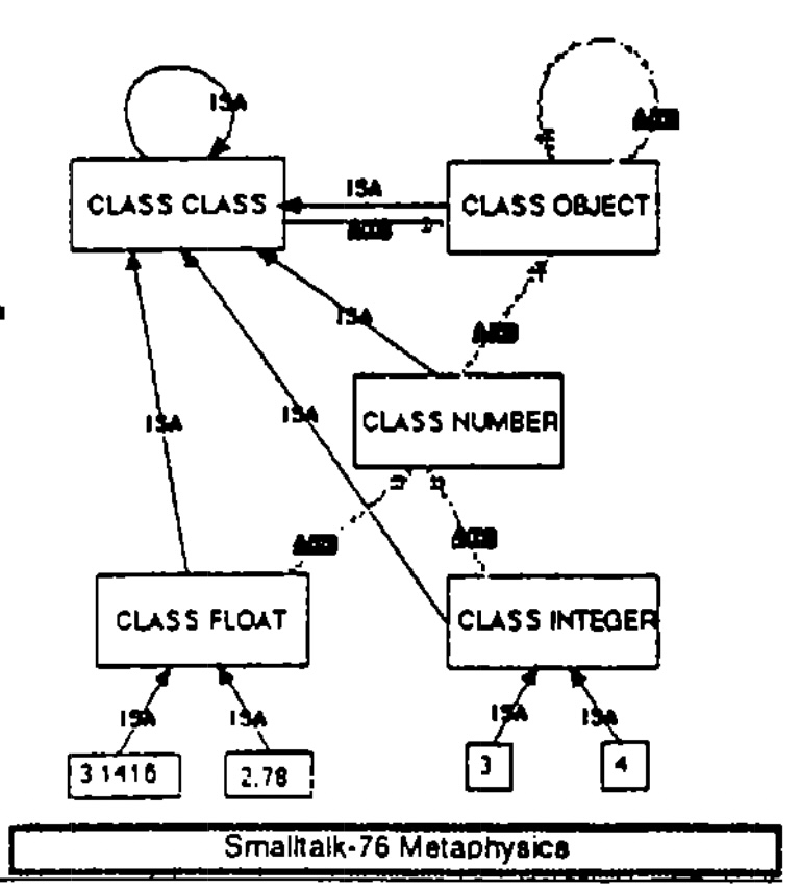
\includegraphics[width=0.8\textwidth]{pictures/smalltalk-76-metaphysics.pdf}
\end{center}
\caption{Smalltalk-76 Metaphyics. From ``\textit{The Early History of
    Smalltalk}'' \cite{kay-history-smalltalk-hopl1993}''. Reproduced
  with permission.}
\label{st-76-metaphysics}
\end{figure}


\subsection{Interpretation} 

The point of these laws, structures, and metaphysics is to execute
Smalltalk programs. Following on from Simula, Smalltalk embodies the idea of
``programming as simulation'': 

\begin{quotation}
\textit{A program execution is regarded as a physical model,
  simulating the behaviour of either a real or an imaginary part of
  the world.}
\end{quotation}
\begin{flushright}
Object-Oriented Programming in BETA \cite{beta}.
\end{flushright}

\noindent For this article, the most important facet of this statement
is the insistence of computation as ``physical model'', a process that
will be embodied via electronic or quantum devices on actual
hardware. (This is in contrast to rather more zipless models of
programming and computation in functional, logical, or quantum
orientation).  For Smalltalk systems, execution is modelled by
exchanges of messages between objects, which is to say a Smalltalk
program.  Traditionally these are modelled as bytecode interpreters:
the methods stored by class objects are arrays of bytes, and the
system implements the methods by interpreting those bytes. (Ingall's
and Kay's HOPL papers give much more details on the evolution of this
design).  The bytecode interpreter is stack based, rather like a
FORTH: arguments are pushed onto a stack: method execution pops its
arguments off the stack and pushes its return value back on.

Figure~\ref{st-76-step} shows the core of the Smalltalk code which
comprises the specification of the Smalltalk-76 bytecodes. This method
reads a byte from the currently execution method, then splits it into
two four-bit ``syllables''. The first syllable, the high bits
(``\textsf{byte|16}'') is used determines the general type of the byte
code -- indeed for many bytecode it determines the entirity of the
operation. The second syllable (``\textsl{lobits}'') can either
identify a particular operation (as in the store, pop, and return
operations in bytecode group~11), or supply a 4-bit operand for an
operation specfied by the first syllable.  See e.g.\ group~6 which
pushes commonly used constants onto the stack, or groups 1--5 which
push values from different types of variables onto the stack.
Groups~9-11 are often called ``extended bytecodes'' because they
provide operations with operands that cannot fit into a 4-bit
syllable, implemented by calling ``\textsf{self nextbyte}'' which
retrieves the nexts byte from the stream.

\begin{figure}[htb]
\begin{center}
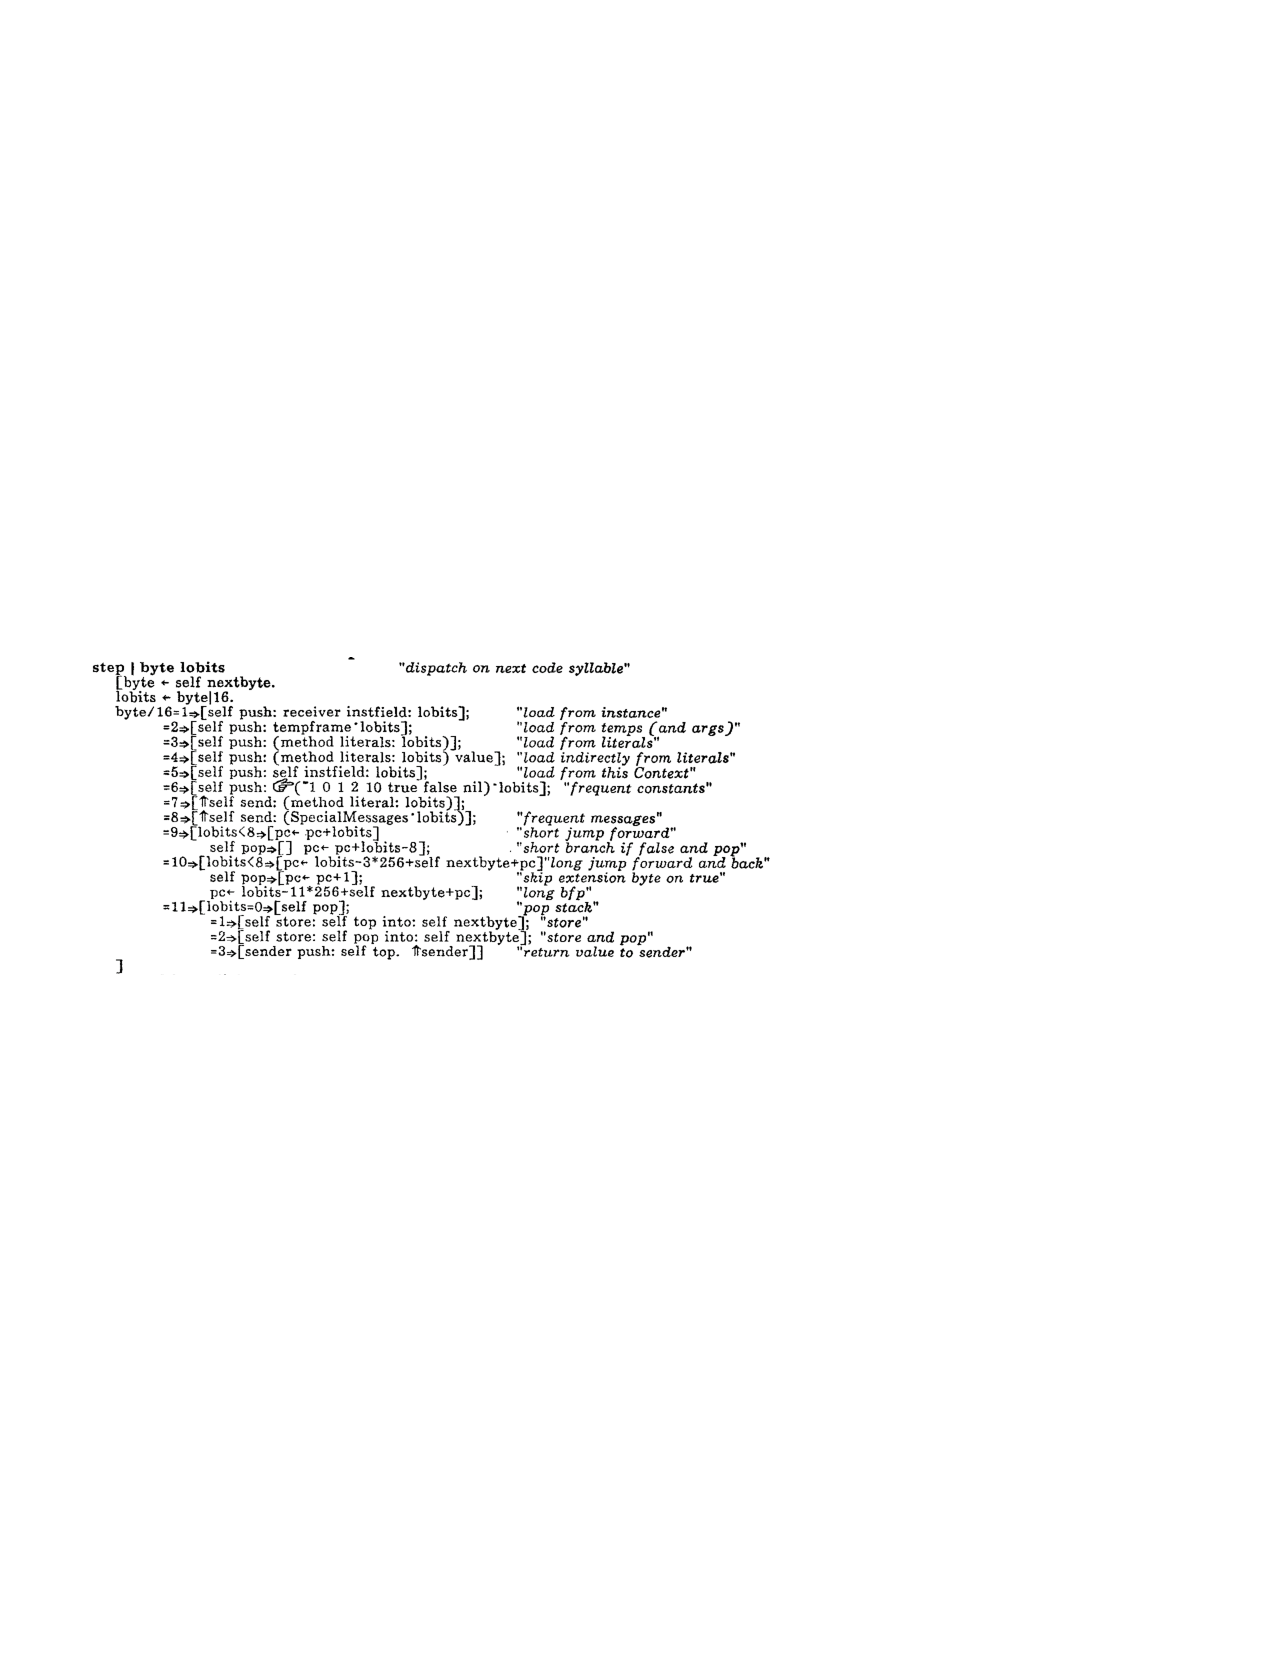
\includegraphics[width=1.0\textwidth]{pictures/st76-step.pdf}
\end{center}
\caption{Smalltalk-76 bytecode decode loop. From ``\textit{The
    Smalltalk-76 Progrmaming System Design and Implementation}''
  \cite{ingalls-smalltalk76-popl1978}''. Reproduced  
  with permission.}
\label{st-76-step}
\end{figure}

Figure~\ref{st-76-store} shows how the store bytecodes are handled,
via a separate ``\textsf{store: val into: field}'' method
Note how the invocation of ``\textsf{store: val into: field}'' in
group~11 in figure~\ref{st-76-step} uses \textsf{nextbyte} to get an
8-bit index of potential store locations.


\begin{figure}[htb]
\begin{center}
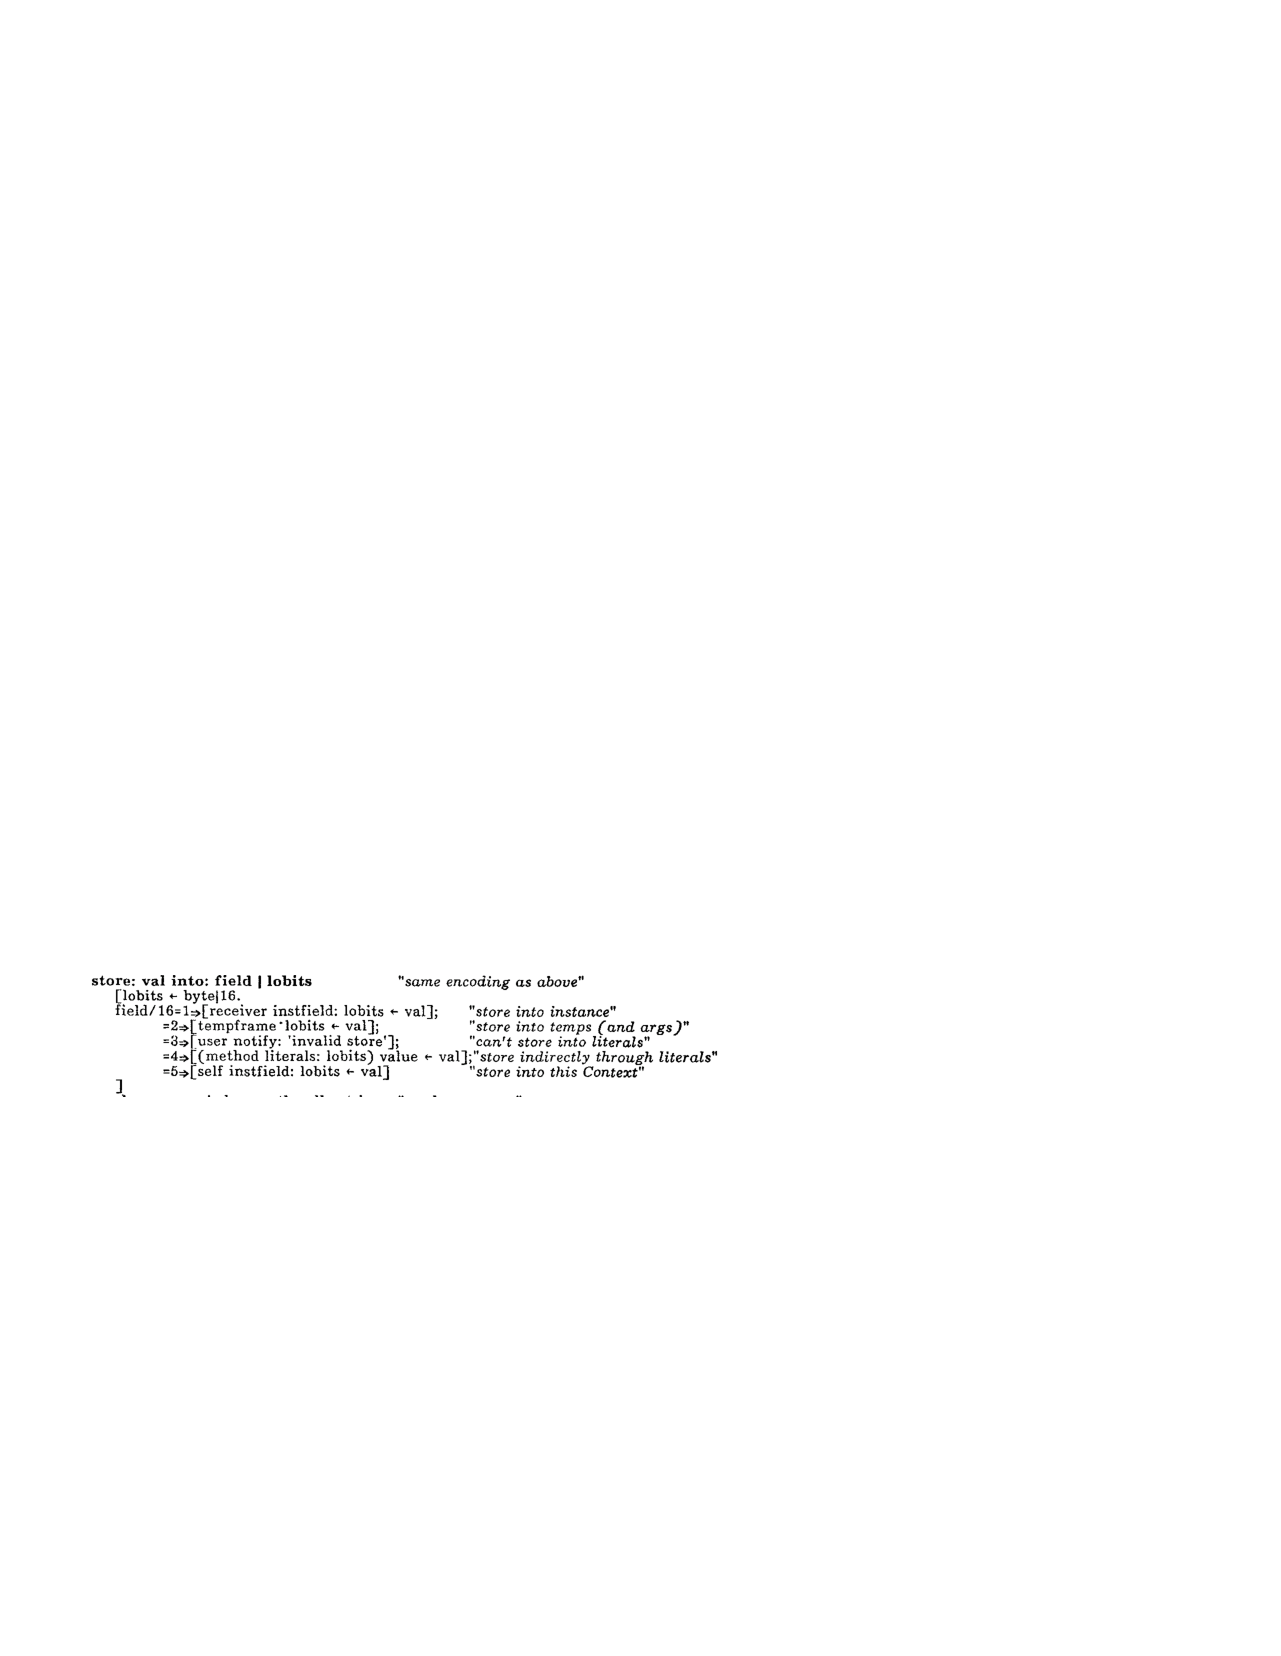
\includegraphics[width=1.0\textwidth]{pictures/st76-store.pdf}
\end{center}
\caption{Smalltalk-76 store bytecode implementation. From ``\textit{The
    Smalltalk-76 Progrmaming System Design and Implementation}''
  \cite{ingalls-smalltalk76-popl1978}''. Reproduced  
  with permission.}
\label{st-76-store}
\end{figure}

Finally figure~\ref{st-76-send} shows the implementation of ``message
sending'' (aka ``dynamic dispatch'' or ``method invocation'' or
``apply'') in Smalltalk-76.  The ``\textsf{send: message}'' method
will be called with an object naming the messagte that has been sent,
i.e.\ the method to be called. The second and fouth line then
implement each stage of the ``\verb+=> ->*+'' rule (one step along the
instance-of relationship, then steps as necessary up the inheritance
relationship). This is called with (a reference to) the reciever
object on the top of the stack. the first line of the method body gets
the top of the stack (``\textsf{self top}'') and then traverses one
step along the instance-of relationship by calling
{``\textsf{class}''} to get that object's class, which will then be
placed into the ``\textsf{class}'' local variable of the
interpreter's method. The class object is then asked to
``\textsf{lookup:}'' the (``\textsf{message}'') in its method
dictionary, and loops over the lookup until the method is found or the
interpreter runs off the top of class ``\textsf{Object}''.   This
lookup involves walking up the inheritance hierarchy from a class to
its superclass --- the code  ``\textsf{class <- class superclass}''
first traverses up from the current ``\textsf{class}'' that has just
been searched to its ``\textsf{superclass}'', and then stores that
superclass into the interpreter's ``\textsf{class}'' local variable.

\begin{figure}[htb]
\begin{center}
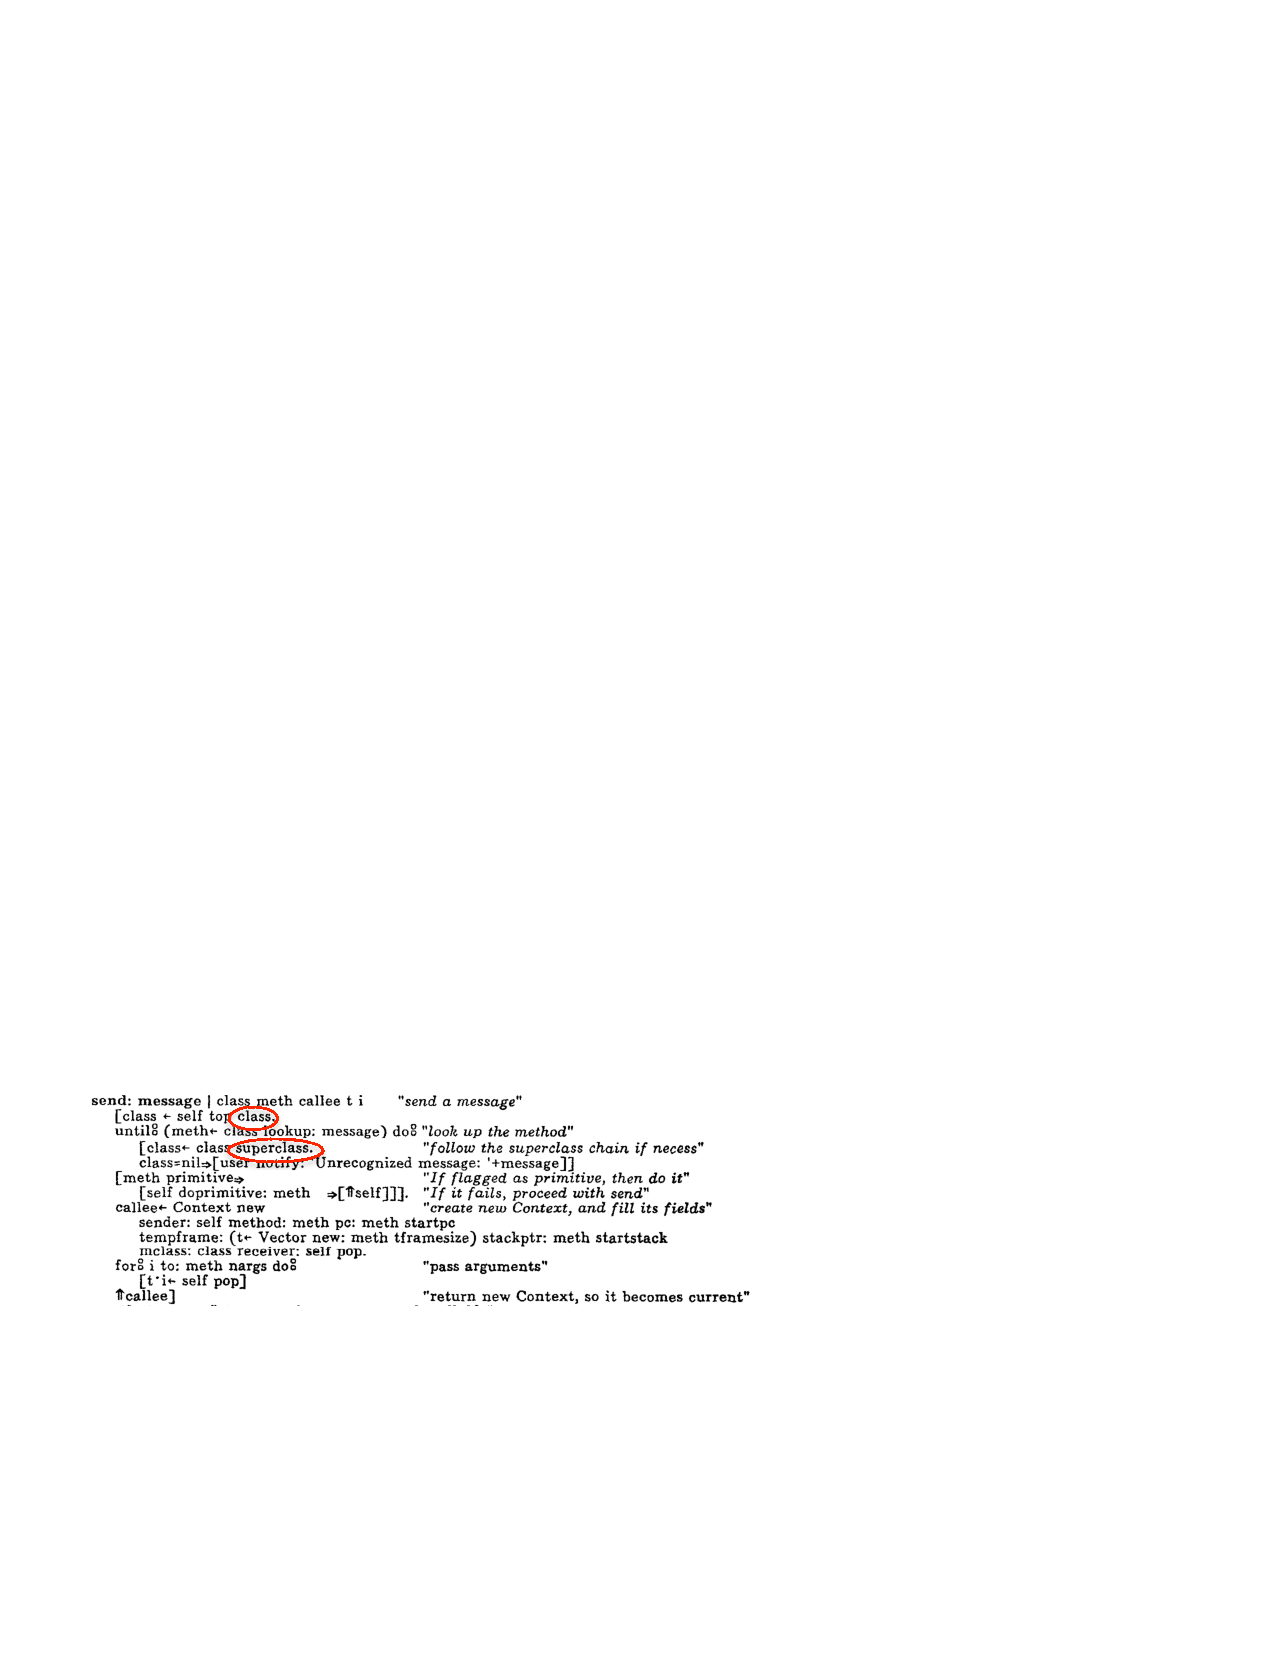
\includegraphics[width=1.0\textwidth]{pictures/st76-send.pdf}
\end{center}
\caption{Smalltalk-76 send bytecode implementation. From ``\textit{The
    Smalltalk-76 Progrmaming System Design and Implementation}''
  \cite{ingalls-smalltalk76-popl1978}''. Reproduced with permission.}
\label{st-76-send}
\end{figure}

